%%==================================================
%% chapter02.tex for BIT Master Thesis
%% modified by yang yating
%% version: 0.1
%% last update: Dec 25th, 2016

%% modified by Meng Chao
%% version: 0.2
%% last update: May 29th, 2017
%%==================================================
\chapter{基于IMU预积分的惯性视觉单目SLAM算法}
\label{chap:VISLAM}
针对第三章提到的单目SLAM算法缺少场景的尺度信息,鲁棒性较差的问题。本章研究一种基于惯性测量单元(IMU)预积分的惯性-视觉单目SLAM算法,在原有基于特征的ORB-SLAM算法基础上,使用预积分算法对IMU数据进行处理,通过非线性优化将IMU预积分结果与视觉传感器进行融合,获取环境的尺度信息并提高单目SLAM算法的鲁棒性。

IMU与视觉数据融合分为松耦合和紧耦合两种方法。松耦合分别通过IMU和图像估计状态变量,之后通过滤波器进行数据融合;紧耦合则将IMU信息与视觉约束放在统一的非线性优化框架下估计状态变量。使用松耦合滤波方法进行数据融合时,状态变量只包含当前状态,不考虑之前的状态。由于受到线性化误差和计算能力的限制,通常只能构建很少的地图点或者采用无结构化的状态向量对地图点进行边缘化。但由于需要对测量的结构化数据进行延时处理,导致状态更新精度下降,且状态变量的边缘化会产生线性化误差和离群值,容易导致滤波器失效;而采用紧耦合非线性优化进行信息融合,状态向量包含随时间滑动的窗口内多个状态或之前的全部状态,使得状态估计更加准确。同时可以引入鲁邦的优化核函数,降低离群值对状态估计的影响。针对本章中IMU与视觉信息融合,由于IMU频率通常在$100-1000Hz$而图像信息大约在$20-60Hz$,无法每次IMU测量后更新状态变量,引入IMU预积分算法估计关键帧之间IMU信息,将预积分得到的状态信息加入非线性优化框架进行状态估计与更新。


%5.1
\section{基于最大后验的惯性-视觉状态估计}
惯性视觉单目SLAM算法主要是通过捷联的IMU与视觉传感器,估计系统的位姿、速度与环境地图点的位置。假设IMU坐标系用$B$表示,相机坐标系用$C$表示,通过预先标定得到相机坐标系到IMU坐标系的坐标变换$\boldsymbol{T}_{BC}$,如图\ref{fig5.1}所示。
\begin{figure}
\centering
%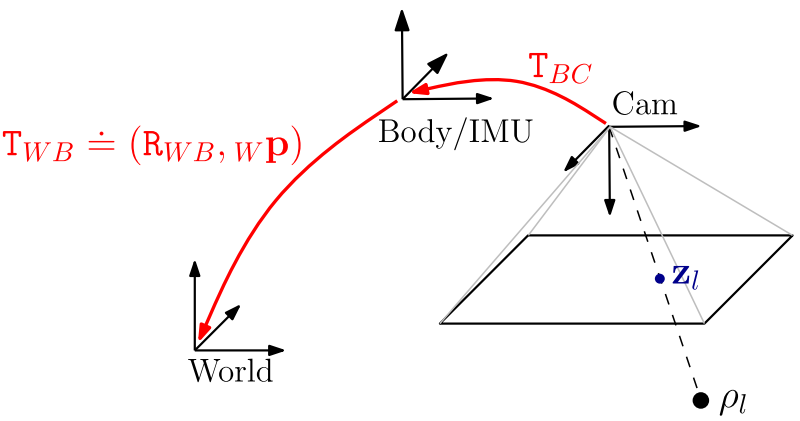
\includegraphics[scale=0.4]{figures/Fig5.1.png}
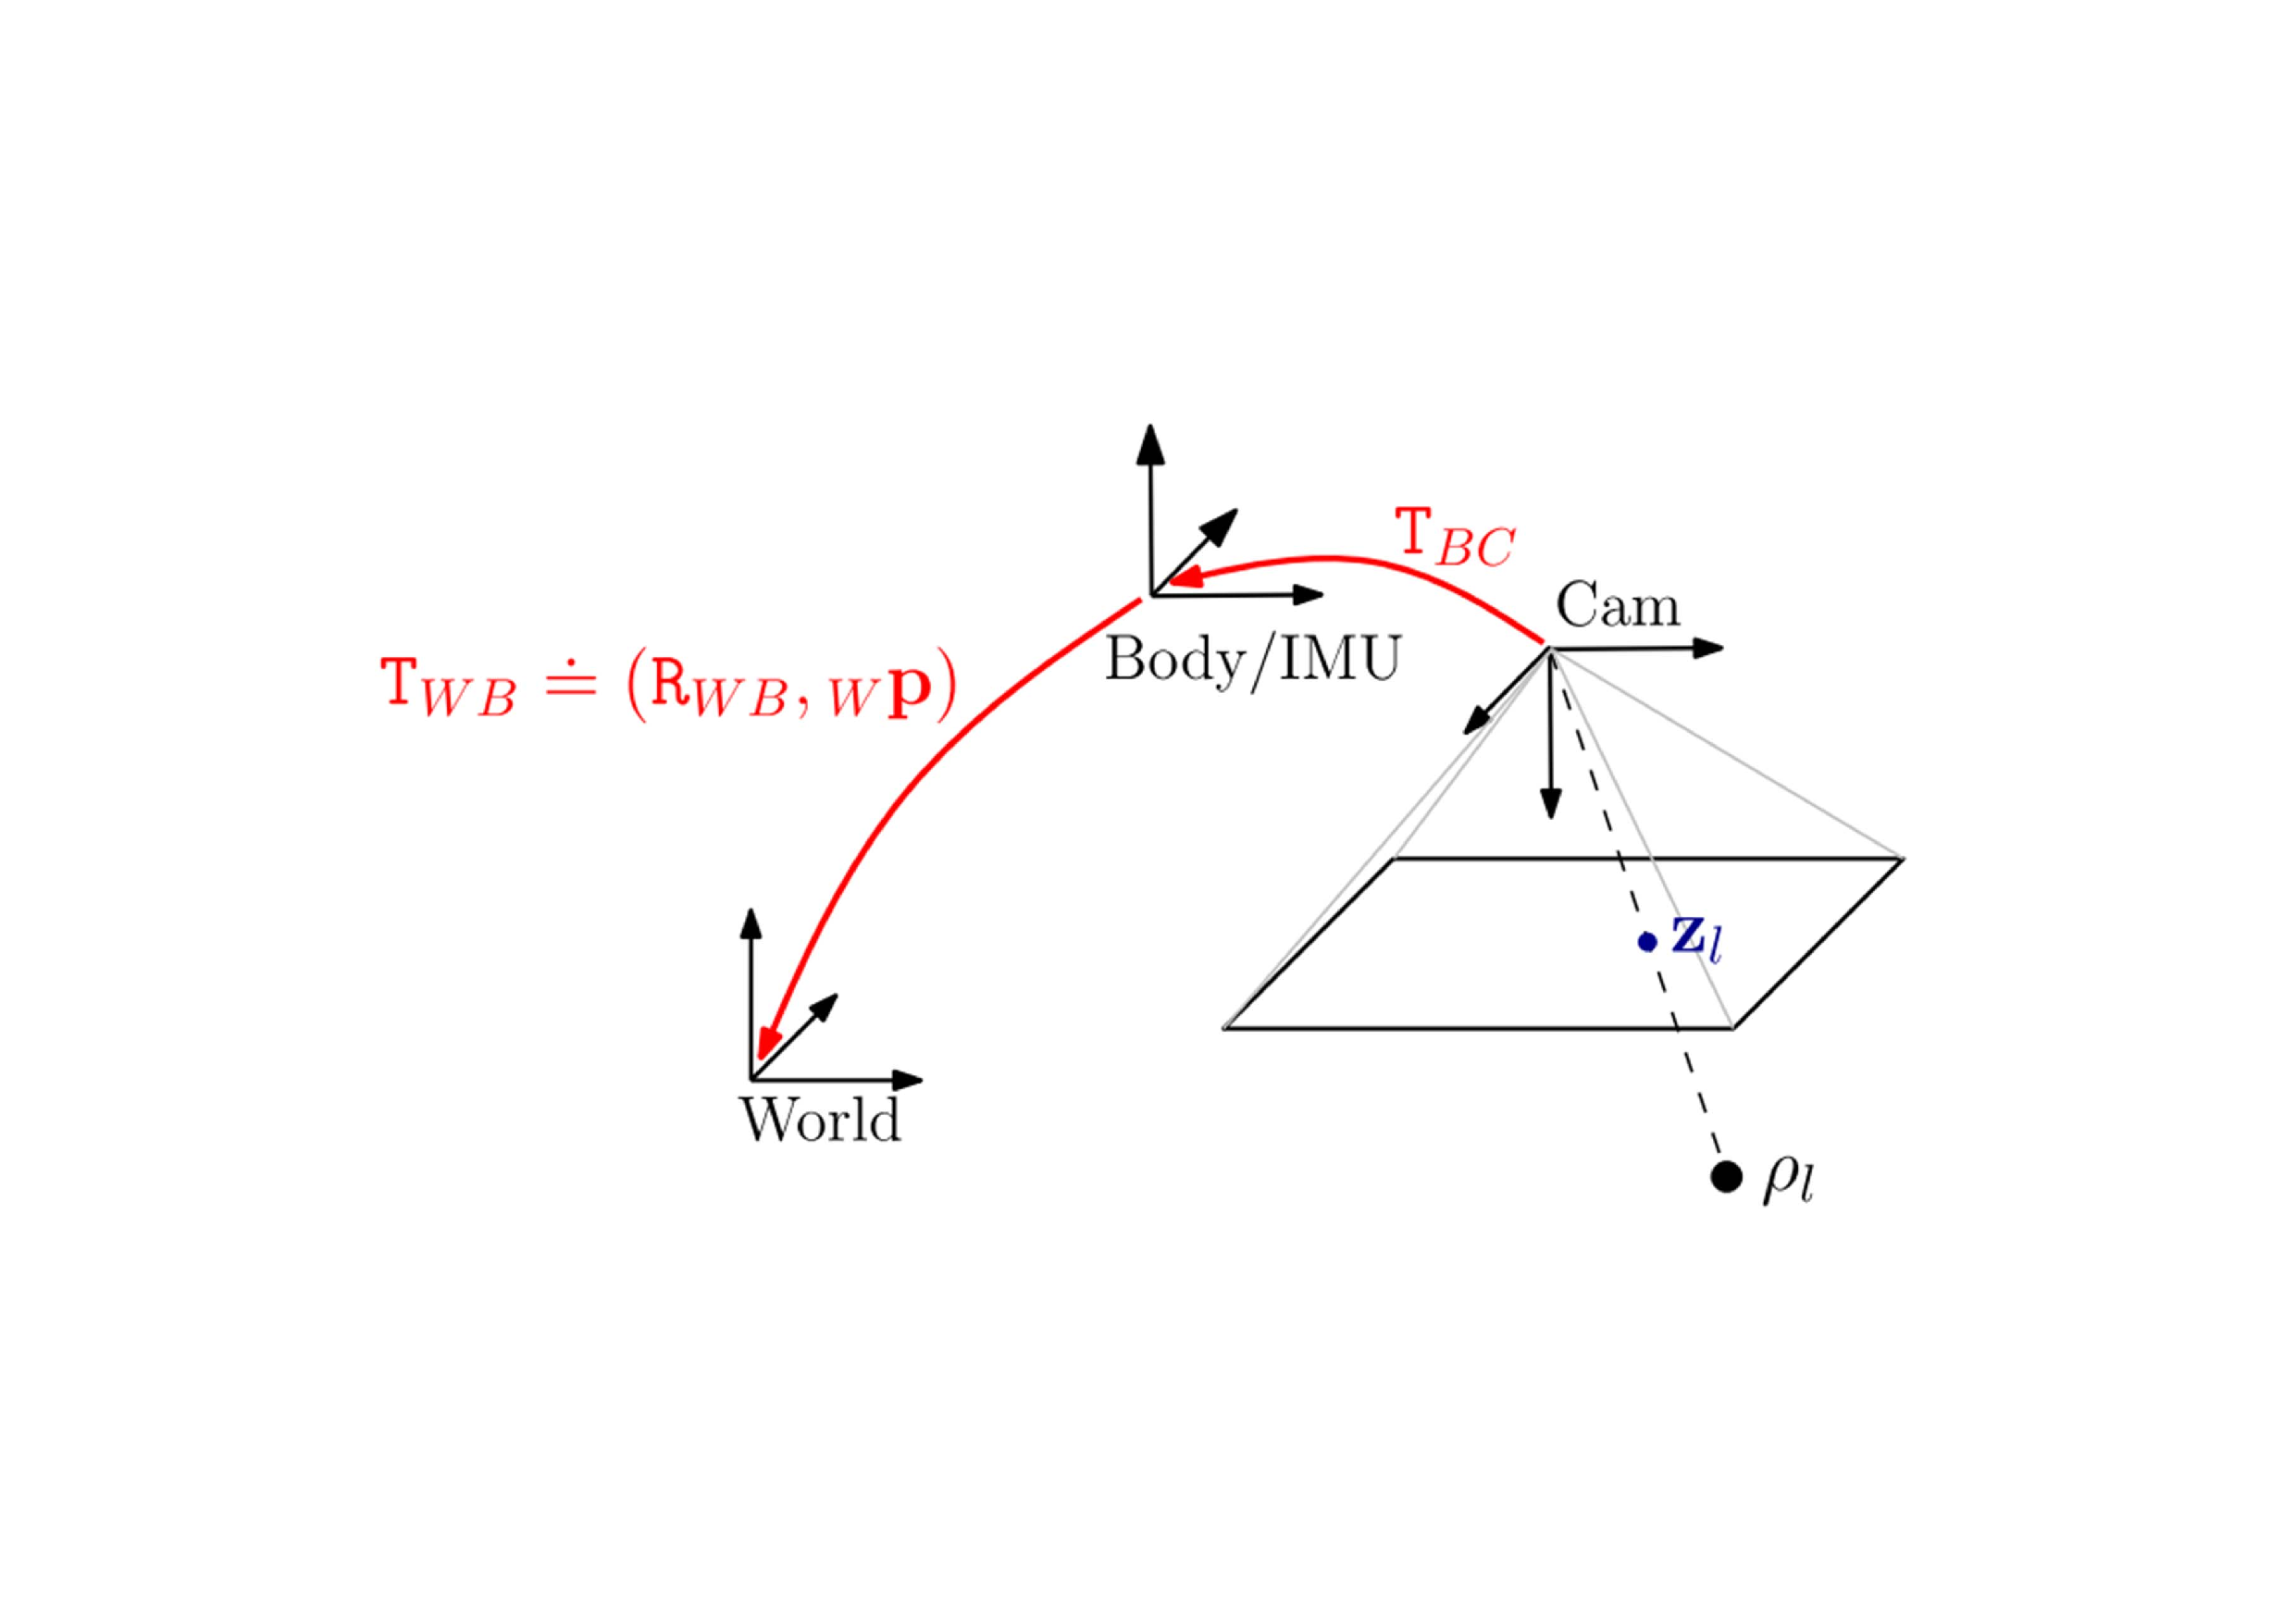
\includegraphics[scale=0.35,angle=-90]{figures/Fig5-1.pdf}
\caption{IMU-相机坐标系变换}
\label{fig5.1}
\end{figure}

在惯性视觉单目SLAM算法中,系统的状态变量可以表示为姿态,位置,速度,IMU偏移
\begin{equation}
\label{equ5.1}
\boldsymbol{x}_i \doteq \left[ \boldsymbol{R}_i,\boldsymbol{p}_i,\boldsymbol{v}_i,\boldsymbol{b}_i \right]
\end{equation}
其中位姿表示在李群$SE(3)$空间下,记作$\left( \boldsymbol{R}_i, \boldsymbol{p}_i \right)$;速度表示在欧式向量空间,记作$\boldsymbol{v}_i \in \mathds{R}^3 $;IMU偏移表示在欧式向量空间下,记作$\boldsymbol{b}_i=[\boldsymbol{b}_i^g \ \boldsymbol{b}_i^a] \in \mathds{R}^6$。

如第三章所述,SLAM问题可以抽象为基于最大后验的状态估计问题。记$k$时刻之前的所有关键帧的集合为$\mathcal{K}_k$,所有关键帧对应状态变量的集合表示为$\mathcal{X}_k \doteq \{\boldsymbol{x}_i\}_{i \in \mathcal{K}_k}$。与纯视觉SLAM问题不同,在惯性视觉单目SLAM算法中输入不仅包括相机图像,还有IMU测量值。第$i$时刻的关键帧图像为$C_i$,图像$C_i$中包括多个地图点$l$在第$i$时刻对应的观测值$z_{il}$。从第$i$时刻到第$j$时刻的两连续关键帧之间的IMU测量值集合为$\mathcal{I}_{ij}$。则$k$时刻之前系统的观测量的集合表示为
\begin{equation}
\label{equ5.2}
Z_k \doteq \{C_i,\mathcal{I}_{ij}\}_{(i,j) \in \mathcal{K}_k}
\end{equation}

将第三章中关于视觉SLAM算法的最大后验状态估计的方法推广到惯性视觉单目SLAM算法中,在给定相机和IMU观测量$Z_k$与先验$p(\mathcal{X}_0)$的情况下,有
\begin{equation}
\label{equ5.3}
\begin{aligned}
p(\mathcal{X}_k | Z_k) & \varpropto p(\mathcal{X}_0)p(Z_k | \mathcal{X}_k) = p(\mathcal{X}_0) \prod\limits_{(i,j) \in \mathcal{K}_k} p \left( C_i,\mathcal{I}_{ij} | \mathcal{X}_k \right) \\
&=p(\mathcal{X}_0) \prod\limits_{(i,j) \in \mathcal{K}_k} p \left( \mathcal{I}_{ij} | x_i,x_j \right) \prod\limits_{i \in \mathcal{K}_k} \prod\limits_{l \in C_i}  p \left( z_{il} | x_i \right)
\end{aligned}
\end{equation}

由于最大后验估计与最小负对数后验估计等价,在传感器观测服从零偏高斯噪声的情况下,对状态变量$\mathcal{X}_k^*$的最大后验估计可以表示为
\begin{equation}
\label{equ5.4}
\begin{aligned}
\mathcal{X}_k^* & = \argmin\limits_{\mathcal{X}_k}- \log_e p(\mathcal{X}_k | Z_k) \\ 
& = \argmin\limits_{\mathcal{X}_k} \left\Vert \boldsymbol{r}_0 \right\Vert_{\boldsymbol{\Sigma}_0}^2+ \sum\limits_{(i,j) \in \mathcal{K}_k}\left\Vert \boldsymbol{r}_{\mathcal{I}_{ij}} \right\Vert_{\boldsymbol{\Sigma}_{ij}}^2+ \sum\limits_{i \in \mathcal{K}_k}\sum\limits_{l \in \mathcal{C}_i} \left\Vert \boldsymbol{r}_{C_{il}} \right\Vert_{\boldsymbol{\Sigma}_{C}}^2
\end{aligned}
\end{equation}
其中$\boldsymbol{r}_0$,$ \boldsymbol{r}_{\mathcal{I}_{ij}}$,$\boldsymbol{r}_{C_{il}}$表示与测量值相关的残差,$\boldsymbol{\Sigma}_0$,$ \boldsymbol{\Sigma}_{ij}$,$\boldsymbol{\Sigma}_C$表示残差对应的协方差矩阵。残差是关于状态变量$\mathcal{X}_k$的方程,用于表示测量值与状态变量$\mathcal{X}_k$给定情况下的预测值之间的误差。公式\eqref{equ5.4}将惯性视觉SLAM问题抽象为关于状态变量$\mathcal{X}_k$的最优估计问题,本章之后的内容介绍如何构建最优估计的目标函数约束和协方差矩阵,将IMU数据耦合到原有的视觉SLAM算法图优化框架中。


%5.2
\section{IMU预积分算法}

\subsection{IMU模型与运动估计}
惯性测量单元(IMU)一般由三轴加速度计和三轴陀螺仪组成,测量传感器相对于惯性坐标系的旋转角速率和加速度。IMU的测量值$\widetilde{\boldsymbol{a}}_B(t)$,$\widetilde{\boldsymbol{\omega}}_{W\!B}(t)$受高斯白噪声$\eta$和传感器偏移$b$的影响,IMU传感器模型如方程\eqref{equ5.5}
\begin{equation}
\label{equ5.5}
\begin{aligned}
\widetilde{\boldsymbol{\omega}}_{W\!B}(t) &= \boldsymbol{\omega}_{W\!B}(t)+\boldsymbol{b}^g(t)+\boldsymbol{\eta}^g(t) \\
\widetilde{\boldsymbol{a}}_B(t) &= \boldsymbol{R}_{W\!B}^T(t)(\boldsymbol{a}_W(t)-\boldsymbol{g}_w)+\boldsymbol{b}^a(t)+\boldsymbol{\eta}^a(t)
\end{aligned}
\end{equation}
其中$\boldsymbol{\omega}_{W\!B}(t) \in \mathds{R}^3$表示在IMU坐标系下IMU坐标系相对于世界坐标系的旋转角速率,$\boldsymbol{a}_W(t) \in \mathds{R}^3$表示相对于世界坐标系下的测量加速度,$\boldsymbol{R}_{W\!B}$表示从IMU坐标系到世界坐标的相对旋转。

为了获取IMU测量的运动信息,根据体动力学模型
\begin{equation}
\label{equ5.6}
\begin{aligned}
\dot{\boldsymbol{R}}_{W\!B} &= \boldsymbol{R}_{W\!B}{\boldsymbol{\omega}}_{W\!B}^{\wedge}\\
\dot{\boldsymbol{v}}_W &= \boldsymbol{a}_W \\
\dot{\boldsymbol{p}}_W &= \boldsymbol{v}_W
\end{aligned}
\end{equation}
其中,${\boldsymbol{\omega}}_{W\!B}^{\wedge}$表示角速率向量的旋转矩阵。对公式\eqref{equ5.6}积分可以得到在$t+\Delta t$时刻的运动状态为
\begin{equation}
\label{equ5.7}
\begin{aligned}
\boldsymbol{R}_{W\!B}(t+\Delta t) &= \boldsymbol{R}_{W\!B}(t)\exp\left( { \left( \int_t^{t+\Delta t} \! \boldsymbol{\omega}_{W\!B}(\tau) d\tau \right)^{\wedge} } \right) \\
\boldsymbol{v}_W(t+\Delta t) &= \boldsymbol{v}_W(t) + \int_t^{t+\Delta t} \! \boldsymbol{a}_W(\tau) d\tau 
\\
\boldsymbol{p}_W(t+\Delta t) &= \boldsymbol{p}_W(t) + \int_t^{t+\Delta t} \! \boldsymbol{v}_W(\tau) d\tau + \iint_t^{t+\Delta t} \! \boldsymbol{a}_W(\tau)d\tau ^2
\end{aligned}
\end{equation}
假设在$t$到$t+\Delta t$时间段内$\boldsymbol{a}_W$和$\boldsymbol{\omega}_{W\!B}$为常量,则公式\eqref{equ5.7}可以表示为
\begin{equation}
\label{equ5.8}
\begin{aligned}
\boldsymbol{R}_{W\!B}(t+\Delta t) &= \boldsymbol{R}_{W\!B}(t) \exp(( \boldsymbol{\omega}_{W\!B}(t)\Delta t )^{\wedge}) \\
\boldsymbol{v}_W(t+\Delta t) &= \boldsymbol{v}_W(t)+\boldsymbol{a}_W(t)\Delta t \\
\boldsymbol{p}_W(t+\Delta t) &= \boldsymbol{p}_W(t)+\boldsymbol{v}_W(t)\Delta t + {1 \over 2} \boldsymbol{a}_W(t)\Delta t^2
\end{aligned}
\end{equation}
将方程\eqref{equ5.5}带入方程\eqref{equ5.8},可以得到运动状态关于IMU测量值$\widetilde{\boldsymbol{\omega}}_{W\!B}$,$\widetilde{\boldsymbol{a}}_B$的函数
\begin{equation}
\label{equ5.9}
\begin{aligned}
\boldsymbol{R}(t+\Delta t) &= \boldsymbol{R}(t)\exp \left( \left(  \left( \widetilde{\boldsymbol{\omega}}_{W\!B}(t)-\boldsymbol{b}^g(t)-\boldsymbol{\eta}^{gd}(t) \right) \Delta t \right)^{\wedge}  \right) \\ 
\boldsymbol{v}(t+\Delta t) &= \boldsymbol{v}(t)+\boldsymbol{g} \Delta t + \boldsymbol{R}(t)(\widetilde{\boldsymbol{a}}(t)-\boldsymbol{b}^a(t)-\boldsymbol{\eta}^{ad}(t))\Delta t \\
\boldsymbol{p}(t+\Delta t) &= \boldsymbol{p}(t)+\boldsymbol{v}(t)\Delta t + {1 \over 2}\boldsymbol{g}\Delta t^2 + {1 \over 2}\boldsymbol{R}(t)(\widetilde{\boldsymbol{a}}(t)-\boldsymbol{b}^a(t)-\boldsymbol{\eta}^{ad}(t))\Delta t^2
\end{aligned}
\end{equation}
为了便于表示,省略方程\eqref{equ5.9}状态变量的坐标系下标。在速度和位置的数值积分中,假设两次测量之间的旋转矩阵$R(t)$为常量,虽然方程\eqref{equ5.9}不是方程\eqref{equ5.7}的精确解,但在IMU采样频率较高时可以认为近似精度足够高,因而在实际应用中采取以上模型近似求解。如果IMU采样速率较低,可以考虑采用更为准确的数值积分近似方法。

\subsection{IMU预积分观测模型}
方程\eqref{equ5.9}可以作为\eqref{equ5.4}最大后验图优化框架的约束,但其中包含需要频繁更新的状态变量。此外,方程\eqref{equ5.9}中涉及到时间$t$和$t+\Delta t$的状态,因此在每次得到新的IMU测量时需要增加状态变量。针对以上问题,采用IMU预积分算法,将连续两帧关键帧之间的IMU观测数据整合为一个包含运动状态的测量信息,如图\ref{fig5.2}所示。
\begin{figure}
\centering
%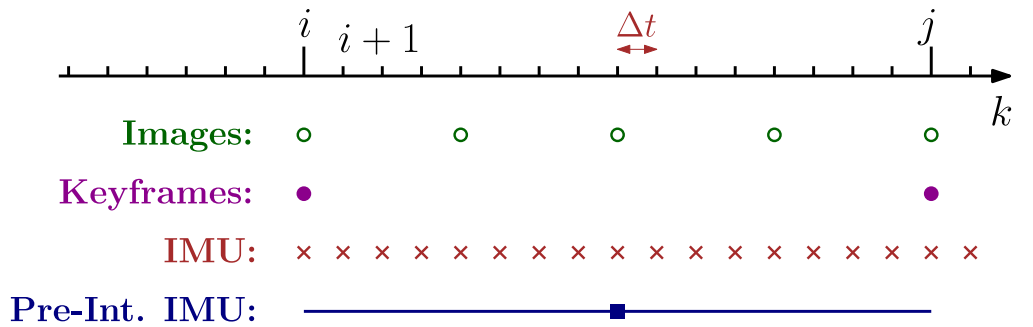
\includegraphics[scale=0.4]{figures/Fig5.2.png}
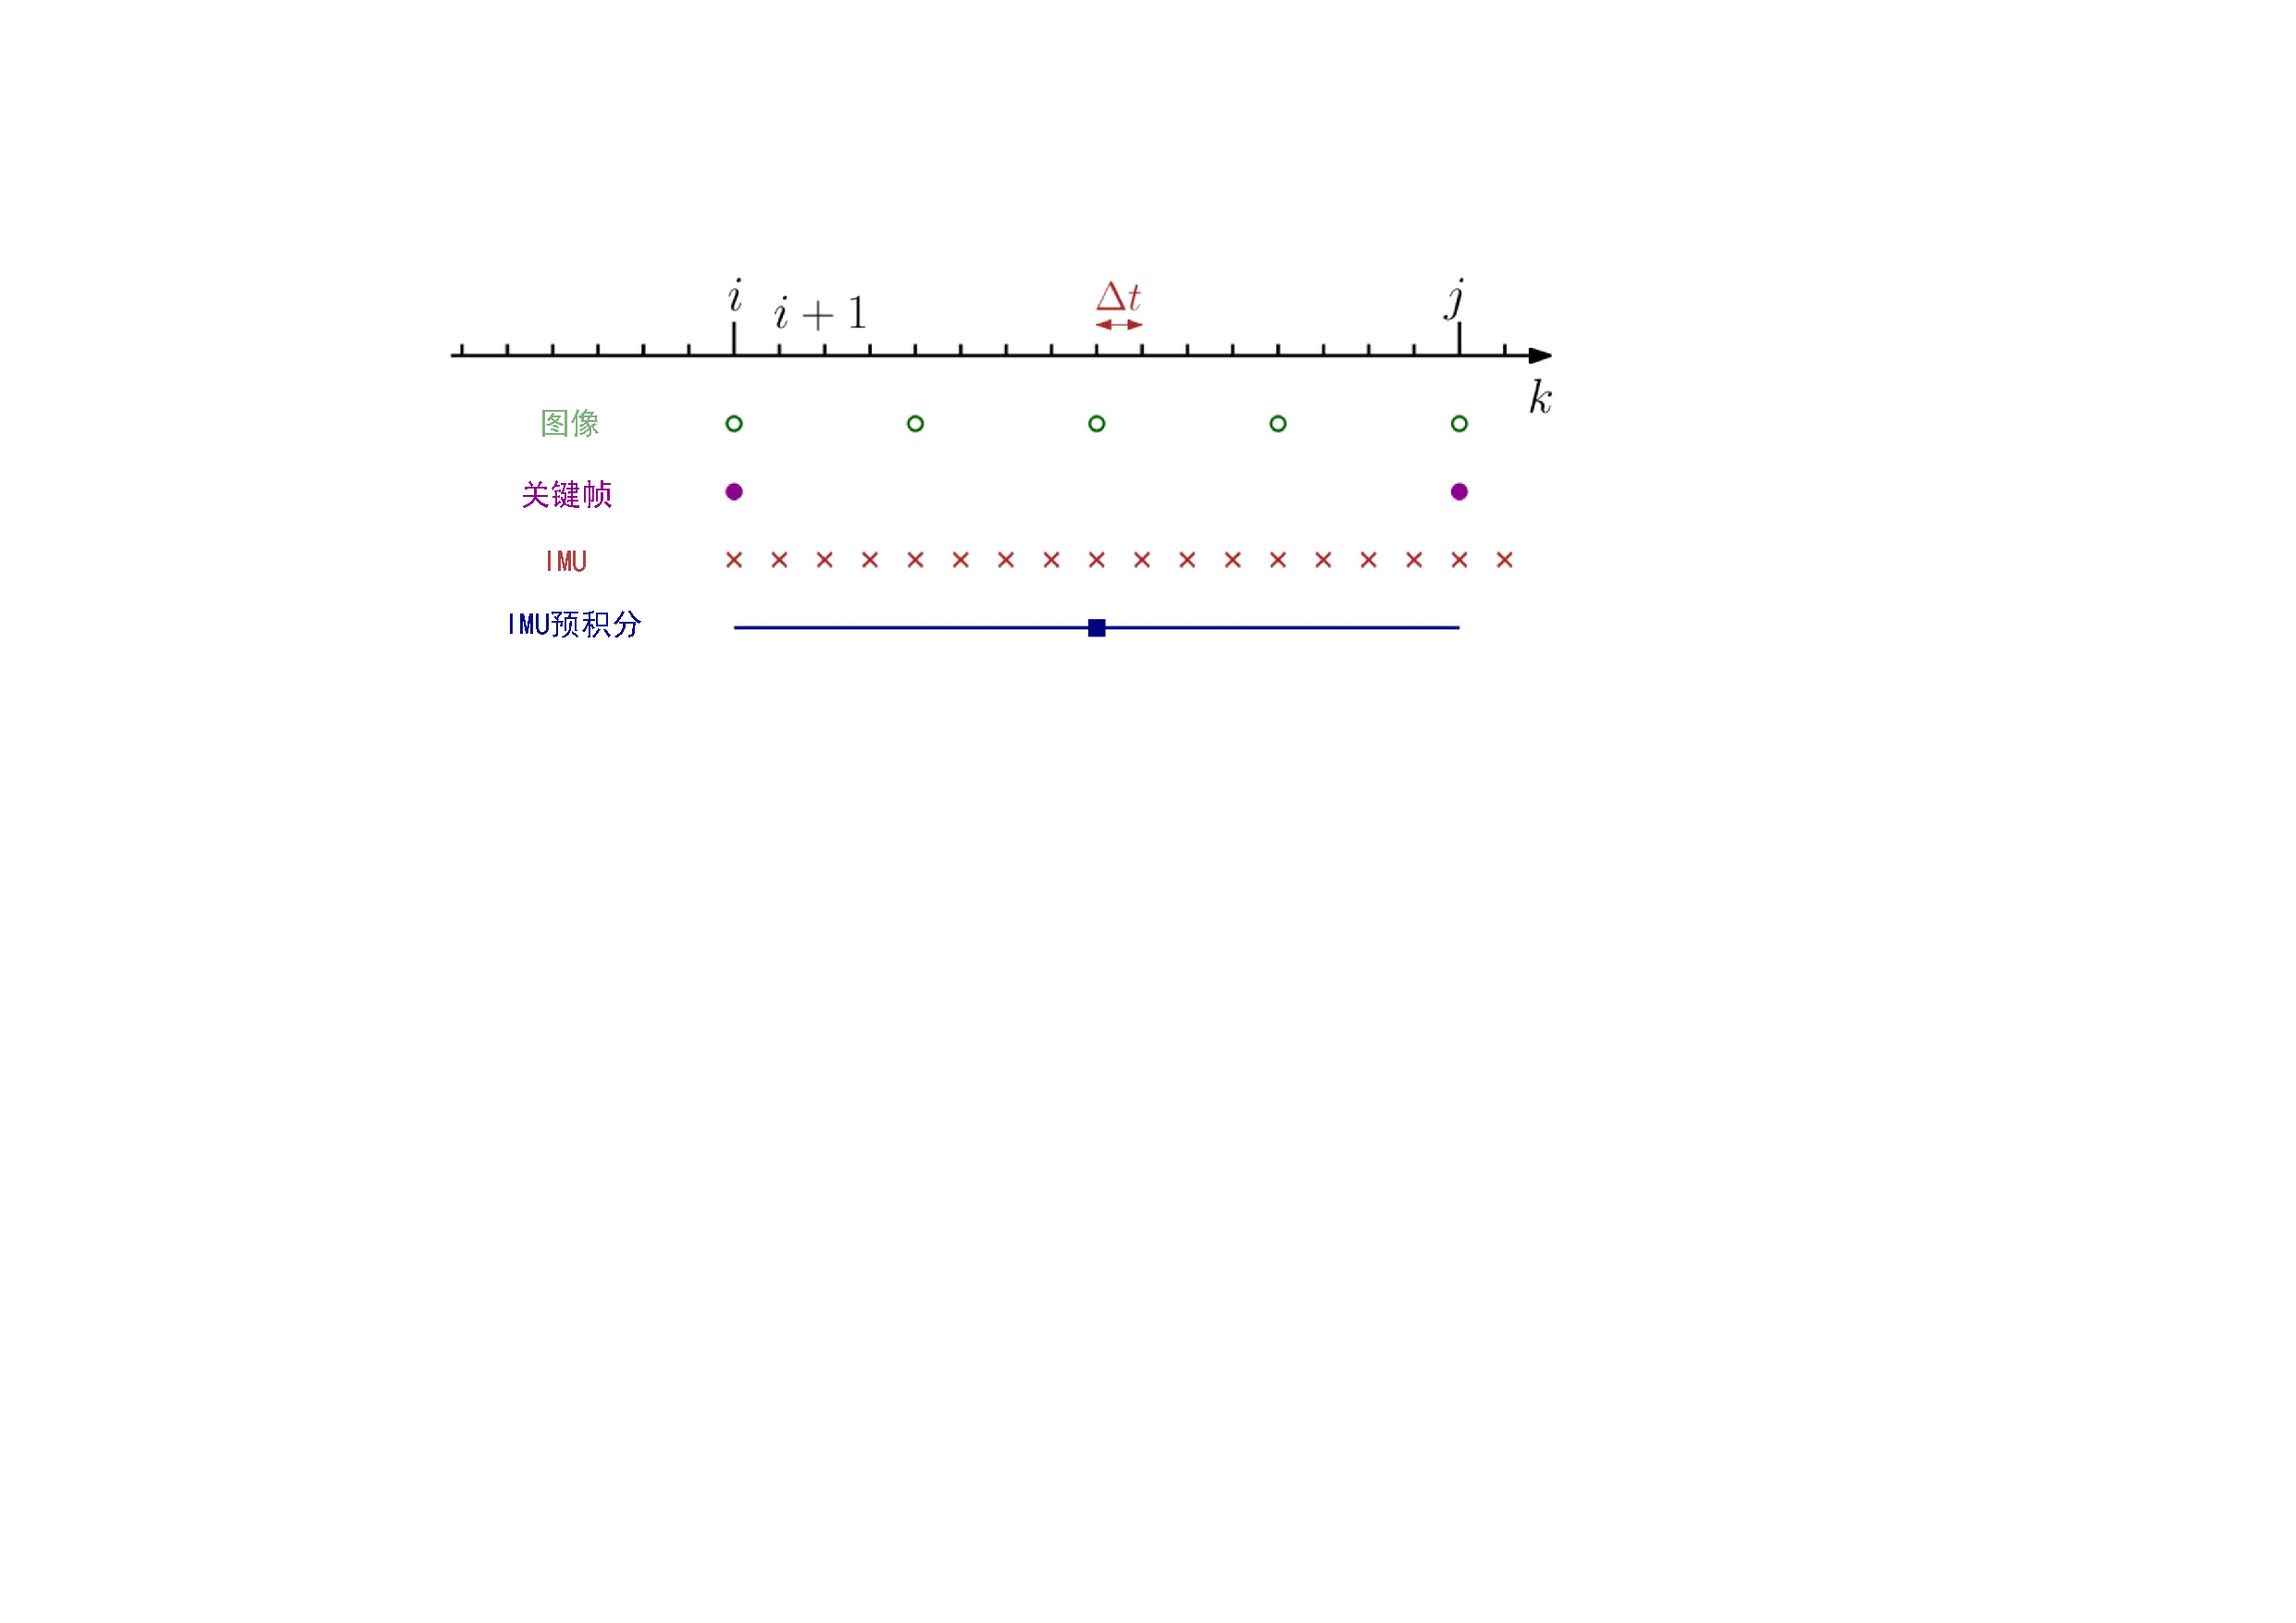
\includegraphics[scale=0.6,angle=-90]{figures/Fig5-2.pdf}
\caption{IMU预积分示意图}
\label{fig5.2}
\end{figure}

假设IMU测量数据与相机图像经过同步处理,对两连续关键帧$i$与$j$之间的所有采样间隔$\Delta t$上的IMU测量数据通过方程\eqref{equ5.9}进行迭代,可以得到
\begin{equation}
\label{equ5.10}
\begin{aligned}
\boldsymbol{R}_j &= \boldsymbol{R}_i \prod\limits_{k=i}^{j-1}\exp \left( \left( \left( \widetilde{\boldsymbol{\omega}}_k - \boldsymbol{b}_k^g-\boldsymbol{\eta}_k^{gd} \right) \Delta t \right)^{\wedge} \right) 
\\ 
\boldsymbol{v}_j &= \boldsymbol{v}_i+\boldsymbol{g} \Delta t_{ij} +  \sum\limits_{k=i}^{j-1}R_k \left( \widetilde{\boldsymbol{a}}_k - \boldsymbol{b}_k^a -\boldsymbol{\eta}_k^{ad} \right)\Delta t
\\
\boldsymbol{p}_j &= \boldsymbol{p}_i + \sum\limits_{k=i}^{j-1} \left[ \boldsymbol{v}_k \Delta t + {1 \over 2}\boldsymbol{g}\Delta t^2 + {1 \over 2}\boldsymbol{R}_k \left( \widetilde{\boldsymbol{a}}_k - \boldsymbol{b}_k^a -\boldsymbol{\eta}_k^{ad} \right)\Delta t^2 \right]
\end{aligned}
\end{equation}
为了便于表示,$(\cdot)_i \doteq (\cdot)(t_i)$,关键帧$i$,$j$之间的时间间隔$\Delta t_{ij} = \sum_{k=i}^{j-1}\Delta t$。方程\eqref{equ5.10}可以用于估计$t_i$到$t_j$时刻之间的运动,但是当方程中的线性化点$t_i$发生变化后,需要重新计算IMU运动信息的数值积分。例如,当姿态$R_i$变化后,从$k=i,...j-1$的所有时刻的姿态,速度和位置都需要重新计算。为了避免重复计算,对方程\eqref{equ5.10}进行变化,定义与$t_i$时刻的位姿和速度无关的相对运动增量
\begin{equation}
\label{equ5.11}
\begin{aligned}
\Delta \boldsymbol{R}_{ij} &\doteq \boldsymbol{R}_i^T \boldsymbol{R}_j = \prod\limits_{k=i}^{j-1}\exp \left( \left( \left( \widetilde{\boldsymbol{\omega}}_k - \boldsymbol{b}_k^g-\boldsymbol{\eta}_k^{gd} \right) \Delta t  \right)^{\wedge} \right) 
\\ 
\Delta \boldsymbol{v}_{ij} &\doteq R_i^T\left( \boldsymbol{v}_j-\boldsymbol{v}_i-\boldsymbol{g}\Delta t_{ij}\right) =  \sum\limits_{k=i}^{j-1} \Delta \boldsymbol{R}_{ik} \left( \widetilde{\boldsymbol{a}}_k - \boldsymbol{b}_k^a -\boldsymbol{\eta}_k^{ad} \right)\Delta t
\\ 
\Delta \boldsymbol{p}_{ij} &\doteq \boldsymbol{R}_i^T \left( \boldsymbol{p}_j-\boldsymbol{p}_i-\boldsymbol{v}_i\Delta  t_{ij} - {1 \over 2} \sum\limits_{k=i}^{j-1} \boldsymbol{g} \Delta t^2 \right) \\
&=  \sum\limits_{k=i}^{j-1} \left[ \Delta \boldsymbol{v}_{ik} \Delta t + {1 \over 2}\Delta \boldsymbol{R}_{ik} \left( \widetilde{\boldsymbol{a}}_k - \boldsymbol{b}_k^a -\boldsymbol{\eta}_k^{ad} \right)\Delta t^2 \right]
\end{aligned}
\end{equation}
其中$\boldsymbol{R}_{ik} \doteq \boldsymbol{R}_i^T \boldsymbol{R}_k$,$\Delta \boldsymbol{v}_{ik} \doteq \boldsymbol{R}_i^T \left( \boldsymbol{v}_k -\boldsymbol{v}_i-\boldsymbol{g}\Delta t_{ik} \right)$。在方程\eqref{equ5.11}中,不同于相对姿态增量$\Delta \boldsymbol{R}_{ij}$,$\Delta \boldsymbol{v}_{ij}$和$\Delta \boldsymbol{p}_{ij}$与实际物理世界中的速度和位置增量并不对应。但这样定义可以使方程\eqref{equ5.11}中$\Delta \boldsymbol{R}_{ij}$,$\Delta \boldsymbol{v}_{ij}$和$\Delta \boldsymbol{p}_{ij}$的右侧表达式直接通过IMU的测量值计算得,而不受$i$时刻的状态和重力加速$\boldsymbol{g}$的影响,避免重复计算。

虽然方程\eqref{equ5.11}可以避免重复计算,但是在每次计算相对状态时,仍需要考虑IMU传感器的偏移$b_i$。在本节之后的推到中,先假设连续两连续关键帧之间的IMU偏移为常量,在下一节中考虑当IMU传感器偏移变化后相对运动增量的补偿。
\begin{equation}
\label{equ5.12}
\boldsymbol{b}_i^g = \boldsymbol{b}_{i+1}^g = \cdots = \boldsymbol{b}_{j-1}^g, \  \boldsymbol{b}_i^a = \boldsymbol{b}_{i+1}^a = \cdots = \boldsymbol{b}_{j-1}^a
\end{equation}

方程\eqref{equ5.11}将关键帧$i$,$j$之间的相对状态(等号左侧)和IMU传感器的测量值(等号右侧)相关联,因而可以将方程\eqref{equ5.11}看做IMU传感器的观测模型。但是,该模型在当前的表示形式下,其观测噪声的不确定性分析较为复杂,无法获取该模型应用于最大后验估计所需要的概率密度函数表达。因而对方程\eqref{equ5.11}进行变换,根据李群与李代数之间的映射关系和性质(见附录),方程\eqref{equ5.11}中IMU旋转观测模型可以表示为
\begin{equation}
\label{equ5.13}
\begin{aligned}
\Delta \boldsymbol{R}_{ij} & \simeq \prod\limits_{k=i}^{j-1} \left[ \exp \left( \left( \left( \widetilde{\boldsymbol{\omega}}_k - \boldsymbol{b}_i^g \right) \Delta t \right)^{\wedge}  \right)  
\exp \left( \left( -J_r^k \boldsymbol{\eta}_k^{gd} \Delta t \right)^{\wedge} \right)\right] \\
&= \Delta \widetilde{\boldsymbol{R}}_{ij} \prod\limits_{k=i}^{j-1}\exp \left( -\Delta \widetilde{\boldsymbol{R}}_{k+1j}^T \left( J_r^k \boldsymbol{\eta}_k^{gd} \Delta t \right)^{\wedge}  \right) \\ 
& \doteq \Delta \widetilde{\boldsymbol{R}}_{ij} \exp \left(  -\delta \boldsymbol{\phi}_{ij} ^{\wedge}  \right)
\end{aligned}
\end{equation}
其中$J_r^k \doteq J_r^k( \left( \widetilde{\boldsymbol{\omega}}_k - \boldsymbol{b}_i^g \right) \Delta t)$,定义IMU旋转预积分为$\Delta \widetilde{\boldsymbol{R}}_{ij} \doteq \prod_{k=i}^j\exp \left( \left( \left( \widetilde{\boldsymbol{\omega}}_k - \boldsymbol{b}_i^g \right) \Delta t \right)^{\wedge}  \right)$,观测模型中的旋转观测噪声为$\delta \boldsymbol{\phi}_{ij}$。

将方程\eqref{equ5.13}带入方程\eqref{equ5.11},利用李代数指数映射的一阶近似(见附录)展开$\exp \left(  -\delta \boldsymbol{\phi}_{ij}^{\wedge}  \right)$,忽略高阶噪声项,则方程\eqref{equ5.11}中的IMU速度观测模型可以表示为
\begin{equation}
\label{equ5.14}
\begin{aligned}
\Delta \boldsymbol{v}_{ij} & \simeq \sum\limits_{k=i}^{j-1} \Delta \widetilde{\boldsymbol{R}}_{ik}\left( \boldsymbol{I}-\delta \boldsymbol{\phi}_{ik}^{\wedge} \right) \left( \widetilde{\boldsymbol{a}}_k - \boldsymbol{b}_i^a \right) \Delta t -\Delta \widetilde{\boldsymbol{R}}_{ik} \boldsymbol{\eta}_k^{ad} \Delta t 
\\ 
& = \Delta \widetilde{\boldsymbol{v}}_{ij} + \sum\limits_{k=i}^{j-1} \left[ \Delta \widetilde{\boldsymbol{R}}_{ik} \left( \widetilde{\boldsymbol{a}}_k - \boldsymbol{b}_i^a \right)^{\wedge} \delta \boldsymbol{\phi}_{ik} \Delta t - \Delta \widetilde{\boldsymbol{R}}_{ik} \boldsymbol{\eta}_k^{ad} \Delta t \right] \\ 
& \doteq  \Delta \widetilde{\boldsymbol{v}}_{ij} - \delta \boldsymbol{v}_{ij}
\end{aligned}
\end{equation}
其中定义IMU的速度预积分为$\Delta \widetilde{\boldsymbol{v}}_{ij} \doteq \sum_{k=i}^{j-1} \Delta \widetilde{\boldsymbol{R}}_{ik} \left( \widetilde{\boldsymbol{a}}_k - \boldsymbol{b}_i^a \right) \Delta t $,IMU速度观测模型的观测噪声为$\delta \boldsymbol{v}_{ij}$。

同理,将方程\eqref{equ5.13},\eqref{equ5.14}带入方程\eqref{equ5.11},利用李代数指数映射的一阶近似,忽略高阶噪声项,则方程\eqref{equ5.11}中的IMU位置观测模型可以表示为
\begin{equation}
\label{equ5.15}
\begin{aligned} 
\Delta \boldsymbol{p}_{ij} & \simeq \sum\limits_{k=i}^{j-1} \left[ (\Delta \widetilde{\boldsymbol{v}}_{ik} - \delta \boldsymbol{v}_{ik}) \Delta t + {1 \over 2} \Delta \widetilde{\boldsymbol{R}}_{ik}\left( \boldsymbol{I}-\delta \boldsymbol{\phi}_{ik}^{\wedge} \right) \left( \widetilde{\boldsymbol{a}}_k - \boldsymbol{b}_i^a  \right) \Delta t^2 - {1 \over 2} \Delta \widetilde{\boldsymbol{R}}_{ik} \boldsymbol{\eta}_k^{ad} \Delta t^2 \right] 
\\ 
& =  \Delta \widetilde{\boldsymbol{p}}_{ij} + \sum\limits_{k=i}^{j-1} \left[ -\delta \boldsymbol{v}_{ik} \Delta t + {1 \over 2} \left( \widetilde{\boldsymbol{a}}_k - \boldsymbol{b}_i^a  \right) ^{\wedge} \delta \boldsymbol{\phi}_{ik} \Delta t^2 - {1 \over 2} \Delta \widetilde{\boldsymbol{R}}_{ik} \boldsymbol{\eta}_k^{ad} \Delta t^2 \right] \\ 
& \doteq \Delta \widetilde{\boldsymbol{p}}_{ij} - \delta \boldsymbol{p}_{ij}
\end{aligned}
\end{equation}
其中,定义IMU位置预积分为$\Delta \widetilde{\boldsymbol{p}}_{ij} \doteq \sum_{k=i}^{j-1} \left( \Delta \widetilde{\boldsymbol{v}}_{ik} \Delta t +  {1 \over 2} \Delta \widetilde{\boldsymbol{R}}_{ik} \left( \widetilde{\boldsymbol{a}}_k - \boldsymbol{b}_i^a  \right) \Delta t^2 \right)$,IMU位置观测模型的观测噪声为$\delta \boldsymbol{p}_{ij}$。

将方程\eqref{equ5.13},\eqref{equ5.14},\eqref{equ5.15}带入方程\eqref{equ5.11}中$\Delta \boldsymbol{R}_{ij}$,$\Delta \boldsymbol{v}_{ij}$,$\Delta \boldsymbol{p}_{ij}$的定义式,可以得到IMU预积分的观测模型
\begin{equation}
\label{equ5.16}
\begin{aligned}
\Delta \widetilde{\boldsymbol{R}}_{ij} &= \boldsymbol{R}_i^T \boldsymbol{R}_j \exp(\delta \boldsymbol{\phi}_{ij}^{\wedge}) 
\\ 
\Delta \widetilde{\boldsymbol{v}}_{ij} &= \boldsymbol{R}_i^T \left(\boldsymbol{v}_j-\boldsymbol{v}_i-\boldsymbol{g}\Delta t_{ij} \right)+\delta \boldsymbol{v}_{ij} 
\\
\Delta \widetilde{\boldsymbol{p}}_{ij} &= \boldsymbol{R}_i^T \left( \boldsymbol{p}_j-\boldsymbol{p}_i-\boldsymbol{v}_i \Delta t_{ij} -{1 \over 2} \boldsymbol{g} \Delta t_{ij}^2 \right) + \delta \boldsymbol{p}_{ij}
\end{aligned}
\end{equation}
方程\eqref{equ5.16}将IMU的测量方程表示为状态变量的函数与观测噪声的和的形式,如果已知IMU观测噪声服从的分布,则可以直接应用在公式\eqref{equ5.4}的最大后验概率估计中,将IMU的测量信息加入视觉SLAM图优化框架,优化求解运动状态变量。因此,需要分析IMU观测噪声$[\delta \boldsymbol{\phi}_{ij}^T,\delta \boldsymbol{v}_{ij}^T,\delta \boldsymbol{p}_{ij}^T]^T$服从的分布,首先考虑旋转观测噪声$\delta \boldsymbol{\phi}_{ij}$,由方程\eqref{equ5.13}可知
\begin{equation}
\label{equ5.17}
\exp \left( -\delta \boldsymbol{\phi}_{ij} \right) \doteq \prod\limits_{k=i}^{j-1} \exp \left( -\Delta \widetilde{\boldsymbol{R}}_{k+1j}^T \left( J_r^k \boldsymbol{\eta}_k^{gd} \Delta t \right)^{\wedge}  \right)
\end{equation}
等号两侧同时去对数,可以得到
\begin{equation}
\label{equ5.18}
\delta \boldsymbol{\phi}_{ij} = -\log \left( \prod\limits_{k=i}^{j-1} \exp \left( -\Delta \widetilde{\boldsymbol{R}}_{k+1j}^T \left( J_r^k \boldsymbol{\eta}_k^{gd} \Delta t \right)^{\wedge}  \right) \right)
\end{equation}
在方程\eqref{equ5.18}中,由于$\boldsymbol{\eta}_k^{gd}$和$\delta \boldsymbol{\phi}_{ij}$是微小噪声,可以认为雅各比矩阵$J_r^k$近似为单位阵,根据李群与李代数指数映射的性质可以近似为
\begin{equation}
\label{equ5.19}
\delta \boldsymbol{\phi}_{ij} \simeq \sum\limits_{k=i}^{j-1} \Delta \widetilde{\boldsymbol{R}}_{k+1j}^T  J_r^k \boldsymbol{\eta}_k^{gd} \Delta t
\end{equation}
由于IMU传感器噪声$\boldsymbol{\eta}_k^{gd}$服从零均值高斯分布,而$\delta \boldsymbol{\phi}_{ij}$是$\boldsymbol{\eta}_k^{gd}$的线性组合,因而$\delta \boldsymbol{\phi}_{ij}$服从零均值高斯分布。对于$\delta \boldsymbol{v}_{ij}$和$\delta \boldsymbol{p}_{ij}$,利用李群与李代数指数映射的性质可以变换为
\begin{equation}
\label{equ5.20}
\begin{aligned}
\delta \boldsymbol{v}_{ij} &\simeq \sum\limits_{k=i}^{j-1} \left[ - \Delta \widetilde{\boldsymbol{R}}_{ik} \left( \widetilde{\boldsymbol{a}}_k - \boldsymbol{b}_i^a  \right) ^{\wedge} \delta \boldsymbol{\phi}_{ik} \delta t + \Delta \widetilde{\boldsymbol{R}}_{ik} \boldsymbol{\eta}_k^{ad} \Delta t   \right] 
\\ 
\delta \boldsymbol{p}_{ij} &\simeq \sum\limits_{k=i}^{j-1} \left[ \delta \boldsymbol{v}_{ik} \Delta t -{1 \over 2} \Delta \widetilde{\boldsymbol{R}}_{ik} \left( \widetilde{\boldsymbol{a}}_k - \boldsymbol{b}_i^a  \right) ^{\wedge} \delta \boldsymbol{\phi}_{ik} \Delta t^2 + { 1 \over 2} \Delta \widetilde{\boldsymbol{R}}_{ik} \boldsymbol{\eta}_k^{ad} \Delta t^2 \right]
\end{aligned}
\end{equation}
方程\eqref{equ5.20}表明$\delta \boldsymbol{v}_{ij}$和$\delta \boldsymbol{p}_{ij}$是加速度计噪声$\boldsymbol{\eta}_k^{ad}$和IMU观测模型旋转噪声$\delta \boldsymbol{\phi}_{ij}$的线性组合,所以$\delta \boldsymbol{v}_{ij}$和$\delta \boldsymbol{p}_{ij}$服从零偏高斯分布。IMU观测模型的噪声分布协方差$\boldsymbol{\Sigma}_{ij}$可以根据IMU传感器高斯白噪声$\boldsymbol{\eta}_k^d \doteq [\boldsymbol{\eta}_k^{gd}, \boldsymbol{\eta}_k^{ad}]^T$计算得到。
\begin{equation}
\label{equ5.21}
\boldsymbol{\eta}_{ij}^{\Delta} \doteq \left[ \delta \boldsymbol{\phi}_{ij}^T, \delta \boldsymbol{v}_{ij}^T, \delta \boldsymbol{p}_{ji}^T \right]^T \sim N \left( \boldsymbol{0}_{9 \times 1}, \boldsymbol{\Sigma}_{ij}  \right)
\end{equation}


\subsection{IMU偏移估计与预积分补偿}
在之前章节对预积分的推导中,都是假设IMU传感器偏移量${\bar{\boldsymbol{b}}^a, \bar{\boldsymbol{b}}^g}$为常量。然而,在实际情况下IMU传感器的偏移在状态估计与优化过程中是变化的,因而需要估计IMU传感器的偏移$\boldsymbol{b}_i^g$、$\boldsymbol{b}_i^a$,对于IMU传感器的偏移的变化,使用"布朗运动"进行建模,有
\begin{equation}
\label{equ5.22}
\dot{\boldsymbol{b}}^g(t) = \boldsymbol{\eta}^{bg}, \ \ \ \dot{\boldsymbol{b}}^a(t) = \boldsymbol{\eta}^{ba}
\end{equation}
对方程\eqref{equ5.22}在两连续关键帧$[t_i,t_j]$时间内积分,可以得到
\begin{equation}
\label{equ5.23}
\boldsymbol{b}_j^g = \boldsymbol{b}_i^g+\boldsymbol{\eta}^{bgd}, \ \ \ \boldsymbol{b}_j^a = \boldsymbol{b}_i^a+\boldsymbol{\eta}^{bad}
\end{equation}
其中,为了表示方便用符号$\boldsymbol{b}_i^g$表示$\boldsymbol{b}^g(t_i)$。定义离散白噪声$\boldsymbol{\eta}^{bgd}$和$\boldsymbol{\eta}^{bad}$,其服从零偏高斯分布,对应的协方差为$\boldsymbol{\Sigma}^{bgd} \doteq \Delta t_{ij} Cov(\boldsymbol{\eta}^{bg}) $,$\boldsymbol{\Sigma}^{bad} \doteq \Delta t_{ij} Cov(\boldsymbol{\eta}^{ba})$。根据方程\eqref{equ5.23}可以构建最大后验概率估计所有关键帧的IMU偏移量,目标优化函数为
\begin{equation}
\label{equ5.24}
\left\Vert \boldsymbol{r}_{\boldsymbol{b}_{ij}} \right\Vert ^2 \doteq \left\Vert \boldsymbol{b}_j^g -\boldsymbol{b}_i^g \right\Vert_{\boldsymbol{\Sigma}^{bgd}}^2 + \left\Vert \boldsymbol{b}_j^a -\boldsymbol{b}_i^a \right\Vert_{\boldsymbol{\Sigma}^{bad}}^2
\end{equation}

当某时刻IMU传感器偏移$\boldsymbol{b}_g$,$\boldsymbol{b}_a$更新后,原有的IMU预积分值会发生变化。一般的处理方法是使用更新后的IMU传感器偏移重新计算预积分,但是增加算法的计算复杂性。另一种做法是根据偏移的变化$\boldsymbol{b} \leftarrow \bar{\boldsymbol{b}}+\delta \boldsymbol{b}$,使用李群与李代数映射的一阶近似(见附录)更新IMU预积分值
\begin{equation}
\label{equ5.25}
\begin{aligned}
\Delta \widetilde{\boldsymbol{R}}_{ij}(\boldsymbol{b}_i^g) &\simeq  \Delta \widetilde{\boldsymbol{R}}_{ij}(\bar{\boldsymbol{b}}_i^g) \exp \left( { \partial \Delta \bar{\boldsymbol{R}}_{ij} \over \partial \boldsymbol{b}^g } \delta \boldsymbol{b}^g \right) 
\\
\Delta \widetilde{\boldsymbol{v}}_{ij}(\boldsymbol{b}_i^g,\boldsymbol{b}_i^a) &\simeq \Delta \widetilde{\boldsymbol{v}}_{ij}(\bar{\boldsymbol{b}}_i^g,\bar{\boldsymbol{b}}_i^a) + { \partial \Delta \bar{\boldsymbol{v}}_{ij} \over \partial \boldsymbol{b}^g } \delta \boldsymbol{b}_i^g + { \partial \Delta \bar{\boldsymbol{v}}_{ij} \over \partial \boldsymbol{b}^a } \delta \boldsymbol{b}_i^a 				
\\
\Delta \widetilde{\boldsymbol{p}}_{ij}(\boldsymbol{b}_i^g,\boldsymbol{b}_i^a) &\simeq \Delta \widetilde{\boldsymbol{p}}_{ij}(\bar{\boldsymbol{b}}_i^g,\bar{\boldsymbol{b}}_i^a) + { \partial \Delta \bar{\boldsymbol{p}}_{ij} \over \partial \boldsymbol{b}^g } \delta \boldsymbol{b}_i^g + { \partial \Delta \bar{\boldsymbol{p}}_{ij} \over \partial \boldsymbol{b}^a } \delta \boldsymbol{b}_i^a 	
\end{aligned}
\end{equation}
其中,雅各比$\{ { \partial \Delta \bar{\boldsymbol{R}}_{ij} \over \partial \boldsymbol{b}^g },{ \partial \Delta \bar{\boldsymbol{v}}_{ij} \over \partial \boldsymbol{b}^g }, \cdots \} $描述了当IMU偏移量发生变化时,预积分如何变化。雅各比的表达式为
\begin{equation}
\label{equ5.26}
\begin{aligned}
{\partial \Delta \bar{\boldsymbol{R}}_{ij} \over \partial \boldsymbol{b}^g } &= - \sum\limits_{k=i}^{j-1} \left[  \Delta \widetilde{\boldsymbol{R}}_{k+1j}(\bar{\boldsymbol{b}}_i)^T J_r^k \Delta t \right] 
\\ 
{\partial \Delta \bar{\boldsymbol{v}}_{ij} \over \partial \boldsymbol{b}^a } &= -\sum\limits_{k=i}^{j-1} \Delta \widetilde{\boldsymbol{R}}_{ij}(\bar{\boldsymbol{b}}_i) \Delta t
\\
{\partial \Delta \bar{\boldsymbol{v}}_{ij} \over \partial \boldsymbol{b}^g } &= -\sum\limits_{k=i}^{j-1} \Delta \widetilde{\boldsymbol{R}}_{ij}(\widetilde{\boldsymbol{a}}_k - \bar{\boldsymbol{b}}_i^a)^{\wedge} {\partial \Delta \bar{\boldsymbol{R}}_{ij} \over \partial \boldsymbol{b}^g } \Delta t
\\
{\partial \Delta \bar{\boldsymbol{p}}_{ij} \over \partial \boldsymbol{b}^a } &= -\sum\limits_{k=i}^{j-1} {3 \over 2} \Delta \widetilde{\boldsymbol{R}}_{ij}(\bar{\boldsymbol{b}}_i) \Delta t^2 
\\
{\partial \Delta \bar{\boldsymbol{p}}_{ij} \over \partial \boldsymbol{b}^g } &= -\sum\limits_{k=i}^{j-1} {3 \over 2} \Delta \widetilde{\boldsymbol{R}}_{ij}(\bar{\boldsymbol{b}}_i) (\widetilde{\boldsymbol{a}}_k - \bar{\boldsymbol{b}}_i^a)^{\wedge} {\partial \Delta \bar{\boldsymbol{R}}_{ij} \over \partial \boldsymbol{b}^g } \Delta t^2
\end{aligned}
\end{equation}

根据方程\eqref{equ5.16}表示的IMU预积分观测模型和公式\eqref{5.21}的观测模型噪声协方差矩阵分析,可以得到方程\eqref{equ5.4}的IMU残差项为$\boldsymbol{r}_{\mathcal{I}_{ij}} \doteq \left[ \boldsymbol{r}_{\Delta \boldsymbol{R}_{ij}}^T,\boldsymbol{r}_{\Delta \boldsymbol{v}_{ij}}^T, \boldsymbol{r}_{\Delta \boldsymbol{p}_{ij}}^T \right]^T \in \mathds{R}^9 $,旋转、速度和位置残差分别为:
\begin{equation}
\label{equ5.27}
\begin{aligned}
\boldsymbol{r}_{\Delta \boldsymbol{R}_{ij}} & \doteq \log \left( \left( \Delta \widetilde{\boldsymbol{R}}_{ij}(\bar{\boldsymbol{b}}_i^g) \exp \left( { \partial \Delta \bar{\boldsymbol{R}}_{ij} \over \partial \boldsymbol{b}^g } \delta \boldsymbol{b}^g \right) \right)^T \boldsymbol{R}_i^T \boldsymbol{R}_j  \right) 
\\
\boldsymbol{r}_{\Delta \boldsymbol{v}_{ij}} & \doteq \boldsymbol{R}_i^T \left(\boldsymbol{v}_j-\boldsymbol{v}_i-\boldsymbol{g}\Delta t_{ij} \right) - \left[ \Delta \widetilde{\boldsymbol{v}}_{ij}(\bar{\boldsymbol{b}}_i^g,\bar{\boldsymbol{b}}_i^a) + { \partial \Delta \bar{\boldsymbol{v}}_{ij} \over \partial \boldsymbol{b}^g } \delta \boldsymbol{b}^g + { \partial \Delta \bar{\boldsymbol{v}}_{ij} \over \partial \boldsymbol{b}^a } \delta \boldsymbol{b}^a  \right] 
\\
\boldsymbol{r}_{\Delta \boldsymbol{p}_{ij}} & \doteq \boldsymbol{R}_i^T \left( \boldsymbol{p}_j-\boldsymbol{p}_i-\boldsymbol{v}_i \Delta t_{ij} -{1 \over 2} \boldsymbol{g} \Delta t_{ij}^2 \right) \\
& - \left[ \Delta \widetilde{\boldsymbol{p}}_{ij}(\bar{\boldsymbol{b}}_i^g,\bar{\boldsymbol{b}}_i^a) + { \partial \Delta \bar{\boldsymbol{p}}_{ij} \over \partial \boldsymbol{b}^g } \delta \boldsymbol{b}^g + { \partial \Delta \bar{\boldsymbol{p}}_{ij} \over \partial \boldsymbol{b}^a } \delta \boldsymbol{b}^a  \right]
\end{aligned}
\end{equation}


%5.3
\section{视觉惯性单目SLAM初始化}
本节研究根据单目SLAM算法获取的一组关键帧和IMU指数映射的测量数据,估计单目SLAM算法轨迹的尺度,重力加速度方向,运动速度和IMU传感器的偏移。本方法需要单目SLAM算法运行一段时间,并假设在此运动期间的所有状态变量是可观的。本初始化方法可以用于任何关键帧在时间上连续的SLAM算法。

视觉惯性单目SLAM算法的初始化可以分为以下几部分:陀螺仪偏移估计;假设加速度计偏移为0的情况下,尺度与重力加速度估计;加速度计偏移估计与尺度、重力加速度估计优化;速度估计。

\subsection{陀螺仪偏移估计}
根据单目SLAM算法连续两帧关键帧的姿态,可以估计陀螺仪偏移。假设陀螺仪偏移在估计时间内保持不变,可以通过最小化单目SLAM算法连续两帧关键帧之间相对姿态和陀螺仪的积分偏差,估计陀螺仪偏移$b_g$。
\begin{equation}
\label{equ5.28}
\argmin\limits_{\boldsymbol{b}_g}\sum\limits_{i=1}^{N-1} \left \Vert Log \left( \left( \Delta \widetilde{\boldsymbol{R}}_{i,i+1} \exp \left( { \partial \Delta \bar{\boldsymbol{R}}_{i,i+1} \over \partial \boldsymbol{b}_g  } \right) \right)^T \boldsymbol{R}_{BW}^i \boldsymbol{R}_{W\!B}^{i+1} \right)  \right \Vert^2
\end{equation}
其中,$N$是选择的一组关键帧的个数,姿态$\boldsymbol{R}_{W\!B}^{(\cdot)}=\boldsymbol{R}_{WC}^{(\cdot)}\boldsymbol{R}_{CB}$是根据单目SLAM关键帧姿态$\boldsymbol{R}_{WC}^{(\cdot)}$和相机-IMU标定参数$\boldsymbol{R}_{CB}$计算得到的。$\Delta \widetilde{\boldsymbol{R}}_{i,i+1}$表示两帧连续关键帧间的IMU陀螺仪旋转预积分值,$\exp \left( { \partial \Delta \bar{\boldsymbol{R}}_{i,i+1} \over \partial \boldsymbol{b}_g  } \right)$是陀螺仪偏移更新后IMU旋转预积分的补偿。采用高斯-牛顿方法求解以上最优问题,估计陀螺仪偏移$\boldsymbol{b}_g$。


\subsection{尺度与重力加速度估计}
完成陀螺仪偏移估计后,可以在IMU的速度预积分与位置预积分增加陀螺仪偏移更新补偿。由于视觉单目SLAM算法初始化时存在尺度信息,因而从相机坐标系$c$到IMU坐标系$B$的坐标变换含有尺度因子$s$:
\begin{equation}
\label{equ5.29}
\boldsymbol{P}_{W\!B} = \boldsymbol{R}_{WC}\ \boldsymbol{P}_{CB} + s\ \boldsymbol{t}_{WC} 
\end{equation}
将方程\eqref{equ5.29}带入IMU预积分观测模型\eqref{equ5.16},忽略加速度计偏移,可以得到
\begin{equation}
\label{equ5.30}
s\ \boldsymbol{t}_{WC}^{i+1} = s\ \boldsymbol{t}_{WC}^i + \boldsymbol{v}_{W\!B}^i \Delta t_{i,i+1}+{1 \over 2} \boldsymbol{g}_W \Delta t_{i,i+1}^2 + \boldsymbol{R}_{W\!B}^i \Delta  \widetilde{\boldsymbol{p}}_{i,i+1} + \left(\boldsymbol{R}_{WC}^i-\boldsymbol{R}_{WC}^{i+1} \right) P_{CB}
\end{equation}
为了降低求解线性方程\eqref{equ5.30}的复杂性,避免求解速度变量,使用方程\eqref{equ5.30}表示三个连续关键帧之间的关系并与方程组\eqref{equ5.16}中的速度预积分方程联立,可以得到
\begin{equation}
\label{equ5.31} 
\begin{bmatrix}
\boldsymbol{\lambda}(i) & \boldsymbol{\beta}(i) \cr 
\end{bmatrix} 
\begin{bmatrix}
s \cr
\boldsymbol{g}_W \cr
\end{bmatrix}
= \boldsymbol{\gamma}(i)
\end{equation}
其中系数矩阵$\boldsymbol{\lambda}(i)$,$\boldsymbol{\beta}(i)$分别为
\begin{equation}
\label{equ5.32}
\begin{aligned}
\boldsymbol{\lambda}(i) &= \left( \boldsymbol{t}_{WC}^{i+1}-\boldsymbol{t}_{WC}^i \right) \Delta t_{i+1,i+2} - \left( \boldsymbol{t}_{WC}^{i+2}-\boldsymbol{t}_{WC}^{i+1} \right)\Delta t_{i,i+1} 
\\ 
\boldsymbol{\beta} (i) &= {1 \over 2} \boldsymbol{I}_{3 \times 3} \left( \Delta t_{i,i+1}^2 \Delta t_{i+1,i+2} + \Delta t_{i+1,i+2}^2 \Delta t_{i,i+1} \right) 
\\ 
\boldsymbol{\gamma} (i) &=  \left( \boldsymbol{R}_{WC}^{i+2} - \boldsymbol{R}_{WC}^{i+1} \right) \boldsymbol{P}_{CB} \Delta t_{i,i+1} - \left( \boldsymbol{R}_{WC}^{i+1} - \boldsymbol{R}_{WC}^{i} \right) \boldsymbol{P}_{CB} \Delta t_{i+1,i+2}  \\ 
& + \boldsymbol{R}_{W\!B}^{i} \Delta \widetilde{\boldsymbol{p}}_{i,i+1} \Delta t_{i+1,i+2} - \boldsymbol{R}_{W\!B}^{i+1} \Delta \widetilde{\boldsymbol{p}}_{i+1,i+2} \Delta t_{i,i+1} 			
\\
& - \boldsymbol{R}_{W\!B}^{i} \Delta \widetilde{\boldsymbol{v}}_{i,i+1} \Delta t_{i,i+1} \Delta t_{i+1,i+2}
\end{aligned}
\end{equation}
对于$N$个连续关键帧,由公式\eqref{equ5.32}可以得到形如$\boldsymbol{A}_{3(N-2)\times4} \  \boldsymbol{x}_{4\times 1} = \boldsymbol{B}_{3(N-2)\times 1}$的超定方程组,通过矩阵奇异值分解(SVD)可以求解轨迹尺度$s$和重力加速度$\boldsymbol{g}_W^*$。需要注意的是,该方程组有4个未知量,$3(N-2)$个方程,因而最少需要4个连续关键帧。


\subsection{加速度计偏移估计}
在之前估计尺度和重力加速度的初始化过程中,忽略IMU加速度计偏移,现在需要考虑加速度计偏移的估计。在估计加速度偏移是,由于之前重力加速度估计的不确定性,如果在方程\eqref{equ5.31}仅仅引入速度计偏移则有可能估计得到病态系统解。为了得到准确的加速度计偏移,引入实际环境重力加速度的大小$G$。假设在惯性坐标系$I$下重力加速度方向为$\boldsymbol{g}_I^{\wedge}= { \begin{bmatrix} 0 & 0 & -1 \cr  \end{bmatrix} ^T }$,上一节中计算得到的世界坐标系下的重力加速方向为$\hat{\boldsymbol{g}}_W = \boldsymbol{g}_W^* / \left\Vert \boldsymbol{g}_W^* \right\Vert$, 可以得到惯性坐标系到世界坐标系的旋转矩阵
\begin{equation}
\label{equ5.33}
\begin{aligned}
& \boldsymbol{R}_{W\!I} = \exp(\hat{\boldsymbol{v}}^{\wedge}\theta)  \\ 
& \hat{\boldsymbol{v}} = { { \hat{\boldsymbol{g}}_I \times \hat{\boldsymbol{g}}_W } \over { \left\Vert \hat{\boldsymbol{g}}_I \times \hat{\boldsymbol{g}}_W   \right\Vert } }\\ 
& \theta = atan2\left( \left\Vert \hat{\boldsymbol{g}}_I \times \hat{\boldsymbol{g}}_W   \right\Vert, \hat{\boldsymbol{g}}_I \cdot \hat{\boldsymbol{g}}_W \right)
\end{aligned}
\end{equation}
则在世界坐标系下,重力加速度向量可以表示为
\begin{equation}
\label{equ5.34}
\boldsymbol{g}_W = \boldsymbol{R}_{W\!I}\hat{\boldsymbol{g}}_IG
\end{equation}
由于$z$轴与重力加速方向平行,$\boldsymbol{R}_{W\!I}$可以用绕$x$、$y$轴的两个旋转角进行参数化。假设存在扰动$\delta \boldsymbol{\theta}$
\begin{equation}
\label{equ5.35}
\begin{aligned}
\boldsymbol{g}_W & = \boldsymbol{R}_{W\!I} \exp (\delta \boldsymbol{\theta}^{\wedge}) \hat{\boldsymbol{g}}_I G 
\\ 
\delta \boldsymbol{\theta} &=
\begin{bmatrix}
\delta \boldsymbol{\theta_{xy}}^T & 0 \cr
\end{bmatrix}^T
\\
\delta \boldsymbol{\theta}_{xy}^T &= 
\begin{bmatrix}
\delta \theta_x & \delta \theta_y \cr
\end{bmatrix}^T
\end{aligned}
\end{equation}
根据李群与李代数指数映射一阶近似,方程\eqref{equ5.35}可以表示为
\begin{equation}
\label{equ5.36}
\boldsymbol{g}_W \simeq \boldsymbol{R}_{W\!I} \hat{\boldsymbol{g}}_I G - \boldsymbol{R}_{W\!I} \hat{\boldsymbol{g}}_I^{\wedge}G\delta \boldsymbol{\theta} 
\end{equation}
将方程\eqref{equ5.36}带入\eqref{equ5.30}有
\begin{equation}
\label{equ5.37}
\begin{aligned}
s \ \boldsymbol{t}_{WC}^{i+1} &= s \ \boldsymbol{t}_{WC}^i +  \boldsymbol{v}_{W\!B}^i \Delta \boldsymbol{t}_{i,i+1} 
- { 1 \over 2} \boldsymbol{R}_{W\!I} \hat{\boldsymbol{g}}_I^{\wedge}G \Delta t_{i,i+1}^2  \delta \boldsymbol{\theta} 
\\
& + \boldsymbol{R}_{W\!B}^i \left( \Delta \widetilde{\boldsymbol{p}}_{i,i+1} + {\partial \Delta \bar{\boldsymbol{p}}_{ij} \over \partial \boldsymbol{b}^a } \boldsymbol{b}_a  \right) +\left( \boldsymbol{R}_{WC}^i - \boldsymbol{R}_{WC}^{i+1} \right) \boldsymbol{P}_{CB} 
\\
& + {1 \over 2} \boldsymbol{R}_{W\!I} \hat{\boldsymbol{g}}_I G \Delta t_{i,i+1}^2
\end{aligned}
\end{equation}
使用方程\eqref{equ5.37}表示三个连续关键帧之间的关系并与方程组\eqref{equ5.31}联立,可以得到关于尺度$s$,重力加速度扰动$\delta \boldsymbol{\theta}$和IMU加速度计偏移$\boldsymbol{b}_a$的线性方程组
\begin{equation}
\label{equ5.38}
\begin{bmatrix}
\boldsymbol{\lambda} (i) & \boldsymbol{\phi} (i) & \boldsymbol{\zeta}  (i) \cr
\end{bmatrix}
\begin{bmatrix}
s \cr \delta \boldsymbol{\theta}_{xy} \cr \boldsymbol{b}_a \cr
\end{bmatrix}
= \boldsymbol{\psi} (i)
\end{equation}
其中线性方程组的系数矩阵$\boldsymbol{\lambda} (i)$与\eqref{equ5.31}相同,系数矩阵$\boldsymbol{\phi}(i)$,$\boldsymbol{\zeta}(i)$,$\boldsymbol{\psi}(i)$为
\begin{equation}
\label{equ5.39}
\begin{aligned}
\boldsymbol{\phi} (i)  &= - \left[ {1 \over 2} \boldsymbol{R}_{W\!I}\hat{\boldsymbol{g}}_I^{\wedge} G \left( \Delta t_{i,i+1}^2 \Delta t_{i+1,i+2}+  \Delta t_{i+1,i+2}^2 \Delta t_{i,i+1} \right) \right]_{(:,1:2)}
\\ 
\boldsymbol{\zeta} (i) &=  \boldsymbol{R}_{W\!B}^{i+1} {\partial \Delta \bar{\boldsymbol{p}}_{i+1,i+2} \over \partial \boldsymbol{b}^a } \Delta t_{i,i+1} + \boldsymbol{R}_{W\!B}^i {\partial \Delta \bar{\boldsymbol{v}}_{i+1,i+2} \over \partial \boldsymbol{b}^a } \Delta t_{i,i+1} \Delta t_{i+1,i+2} \\
 &- \boldsymbol{R}_{W\!B}^{i} {\partial \Delta \bar{\boldsymbol{p}}_{i,i+1} \over \partial \boldsymbol{b}^a } \Delta t_{i+1,i+2} 
\\  
\boldsymbol{\psi} (i) & = \left( \boldsymbol{R}_{W\!B}^{i} - \boldsymbol{R}_{W\!B}^{i+1} \right) \boldsymbol{P}_{CB} \Delta t_{i+1,i+2} + \boldsymbol{R}_{W\!B}^{i} \widetilde{\boldsymbol{p}}_{i,i+1} \Delta t_{i+1,i+2} \\
& - \left( \boldsymbol{R}_{W\!B}^{i+1} - \boldsymbol{R}_{W\!B}^{i+2} \right) \boldsymbol{P}_{CB} \Delta t_{i,i+1} - \boldsymbol{R}_{W\!B}^{i+1} \widetilde{\boldsymbol{p}}_{i+1,i+2} \Delta t_{i,i+1} \\ 
& - \boldsymbol{R}_{W\!B}^{i} \widetilde{\boldsymbol{v}}_{i,i+1}  \Delta t_{i,i+1} \Delta t_{i+1,i+2} \\
& - {1 \over 2} \boldsymbol{R}_{W\!I} \hat{\boldsymbol{g}}_I G \left( \Delta t_{i,i+1}^2 \Delta t_{i+1,i+2} + \Delta t_{i+1,i+2}^2 \Delta t_{i,i+1} \right)
\end{aligned}
\end{equation}
其中,$[\cdot]_{:,1:2}$表示矩阵的前两列,这是因为重力加速度扰动$\delta \boldsymbol{\theta}$第三项为0。对于N个连续关键帧,方程\eqref{equ5.38}是形如$\boldsymbol{A}_{3(N-2)\times 6}\  \boldsymbol{x}_{6\times 1} = \boldsymbol{B}_{3(N-2)\times 1}$的超定线性方程组,可以通过对系数矩阵进行奇异值分解(SVD)求解尺度$s$,重力加速度扰动$\delta \boldsymbol{\theta}$和IMU加速度计偏移$\boldsymbol{b}_a$。该方程组有6个未知量,$3(N-2)$个方程,因而最少需要4个连续关键帧。


\subsection{速度估计与重定位后的IMU偏移估计}
在方程\eqref{equ5.30},\eqref{equ5.37}求解尺度,重力加速度和IMU加速度计偏移时,通过三个连续关键帧之间的关系来消去速度变量。在进行速度估计时,可以利用已知的尺度,重力加速度和IMU加速度计偏移,直接带入方程\eqref{equ5.37}直接求解关键帧的速度状态$\boldsymbol{v}_{W\!B}^i$。

当算法运行过程中出现跟踪失效丢失,经过一段时间重定位并成功时,由于IMU传感器偏移发生变化,需要重新估计当前IMU传感器偏移。首先可通过方程\eqref{equ5.28}估计陀螺仪偏移$\boldsymbol{b}_g$。估计加速度计偏移时,由于轨迹尺度$s$和重力加速度$\boldsymbol{g}_W$已知且不变,因而只需要带入方程\eqref{equ5.38}即可。

\section{本章小结}




\iffalse
A 3D rigid body transform $G{\rm{ }} \in {\rm{ }}SE(3)$  denotes rotation and translation in 3D,  i.e. is defined by

\begin{equation}
G=\left(
    \begin{array}{cc}
      R & t \\
      0 & 1 \\
    \end{array}
  \right)
    \ with
    \ R\in SO(3)
    \ and
    \ t\in {\mathbb{R}}^{3}
\end{equation}
SE(3) and SO(3) is the concept of elements of Lie-Algebras.

We define the 3D projective warp function $\omega $, which projects an image point ${\bf{p}}$ and its inverse depth ${\bf{d}}$ into a by $\xi $ transformed camera frame.

\begin{equation}
\begin{split}
\omega(p,d,\xi):= \left(
                     \begin{array}{c}
                       x^{'}/z^{'} \\
                       y^{'}/z^{'} \\
                       1/z^{'} \\
                     \end{array}
                   \right) \ with \\
                   \left(
                     \begin{array}{c}
                       x^{'} \\
                       y^{'} \\
                       z^{'} \\
                       1 \\
                     \end{array}
                   \right):=\!exp_{\!se(\!3\!)}(\xi)
                   \left(
                     \begin{array}{c}
                       p_{x}/d \\
                       p_{y}/d  \\
                       1/d  \\
                       1 \\
                     \end{array}
                   \right)
\end{split}
\end{equation}

A 3D similarity transform   denotes rotation, scaling and translation, i.e. is defined by

\begin{equation}
S=\left(
    \begin{array}{cc}
      sR & t \\
      0 & 1 \\
    \end{array}
  \right)
  \ with
  \ R\in SO(3),t\in {\mathbb{R}}^{3}
  \ and \ s\in {\mathbb{R}}^{+}
\end{equation}

As for rigid body transformations, a minimal representation is given by elements of the associated Lie-algebra $\xi  \in sim(3)$, which now have an additional degree of freedom, that is $\xi\in {\mathbb{R}}^{7}$.

\fi



